\documentclass[tikz,border=5pt]{standalone}
\usepackage{amssymb}
\usepackage{amsfonts}
\usepackage{mathrsfs}
\usepackage{amsthm}
\usepackage{amsmath}
\usepackage{xcolor}
\usepackage{hyperref}
\usepackage{libertinus}
\usepackage{dsfont}
\usepackage{bm}
\usepackage{enumitem}
\usepackage{caption}
\usepackage{subcaption}
\usepackage{tikz}
\usepackage{quiver}

\newcommand{\R}{\mathbb{R}}
\newcommand{\C}{\mathbb{C}}
\newcommand{\N}{\mathbb{N}}
\newcommand{\Z}{\mathbb{Z}}
\newcommand{\Q}{\mathbb{Q}}

\newcommand{\id}{\operatorname{id}}

% differentials and derivatives
\renewcommand{\d}{\mathrm{d}}
\newcommand{\dd}{\,\d}
\newcommand{\pddf}[2]{\frac{\partial#1}{\partial#2}}
\newcommand{\ddt}{\frac{\d }{\d t}}
\newcommand{\ddtz}{\left.\ddt\right|_{t=0}}

\begin{document}
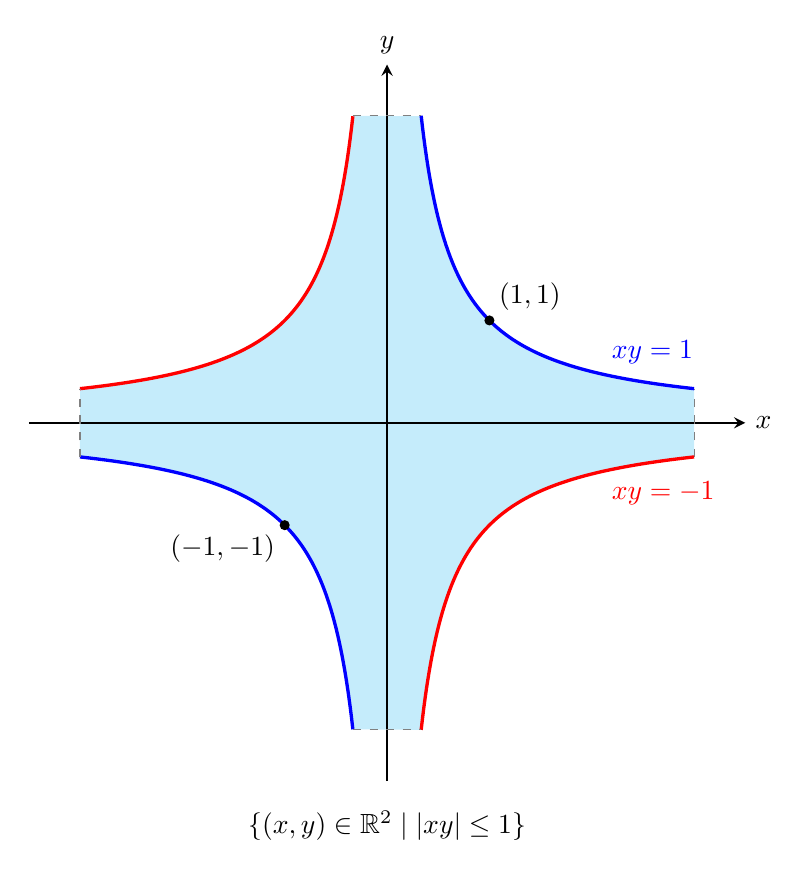
\begin{tikzpicture}[scale=1.3, >=stealth]

    % The window is [-\L,\L]^2; the arms of the star are cut off at its edges,
    % where the hyperbolas xy = \pm 1 reach the height 1/\L.
    \def\L{3}
    \def\e{0.333333}

    % The region |xy| <= 1, traversed counterclockwise
    \fill[cyan!45, opacity=0.5]
        (\L,-\e) -- (\L,\e)
        -- plot[domain=\L:\e, samples=200, variable=\x] (\x, {1/\x})
        -- (-\e,\L)
        -- plot[domain=-\e:-\L, samples=200, variable=\x] (\x, {-1/\x})
        -- (-\L,-\e)
        -- plot[domain=-\L:-\e, samples=200, variable=\x] (\x, {1/\x})
        -- (\e,-\L)
        -- plot[domain=\e:\L, samples=200, variable=\x] (\x, {-1/\x})
        -- cycle;

    % Axes
    \draw[->, thick] (-\L-0.5,0) -- (\L+0.5,0) node[right] {$x$};
    \draw[->, thick] (0,-\L-0.5) -- (0,\L+0.5) node[above] {$y$};

    % Boundary: the hyperbolas xy = 1 ...
    \draw[blue, very thick]
        plot[domain=\e:\L, samples=200, variable=\x] (\x, {1/\x});
    \draw[blue, very thick]
        plot[domain=-\L:-\e, samples=200, variable=\x] (\x, {1/\x});
    % ... and xy = -1
    \draw[red, very thick]
        plot[domain=-\L:-\e, samples=200, variable=\x] (\x, {-1/\x});
    \draw[red, very thick]
        plot[domain=\e:\L, samples=200, variable=\x] (\x, {-1/\x});

    % The arms are unbounded; the dashed segments are only where the picture stops
    \draw[gray, dashed] (\L,-\e) -- (\L,\e);
    \draw[gray, dashed] (-\L,-\e) -- (-\L,\e);
    \draw[gray, dashed] (-\e,\L) -- (\e,\L);
    \draw[gray, dashed] (-\e,-\L) -- (\e,-\L);

    % Curve labels
    \node[blue, anchor=south west] at (2.1,{1/2.1}) {$xy=1$};
    \node[red, anchor=north west] at (2.1,{-1/2.1}) {$xy=-1$};

    % Unit hyperbola corners
    \fill (1,1) circle (1.4pt) node[anchor=south west] {$(1,1)$};
    \fill (-1,-1) circle (1.4pt) node[anchor=north east] {$(-1,-1)$};

    \node[anchor=north] at (0,-\L-0.7)
        {$\{(x,y)\in\R^2 \mid |xy|\leq 1\}$};

\end{tikzpicture}
\end{document}
